% -*- mode: LaTex; outline-regexp: "\\\\section\\|\\\\subsection";fill-column: 80; -*-
\documentclass[12pt]{article}
\usepackage[longnamesfirst]{natbib}
\usepackage[usenames]{color}
\usepackage{amssymb}
\usepackage{graphicx}
\usepackage{parsetree}
% http://www.ling.helsinki.fi/kit/2002s/ctl230/LaTeX/parsetree.sty
% http://www.essex.ac.uk/linguistics/external/clmt/latex4ling/trees/parsetree/
\input{../../standard}

% --- Margins
\setlength{\oddsidemargin}{0.25in}
\setlength{\textwidth}{6in}

\setlength{\topmargin}{-.10in}  % where to start head, relative to 1 inch
\setlength{\headheight}{.1in}   % reserved for the head
\setlength{\textheight}{8.5in}  % height of the body of the text
\setlength{\headsep}{.4in}      % separation of body and head

% --- Separation of displayed math from adjoining text
\setlength{\abovedisplayskip 0.1in}
\setlength{\belowdisplayskip 0.1in}

% --- Paragraph split
\setlength{\parskip}{0.00in}

% --- Line spacing
\renewcommand{\baselinestretch}{1.7}  % 1.7 gives 25 lines per page

% --- Hypthenation
\sloppy  % fewer hyphenated
\hyphenation{stan-dard}
\hyphenation{among}

% --- Customized commands, abbreviations
\newcommand{\TIT}{{\it  {\tiny  Testing Multiple Endpoints}}}
\newcommand{\hypn}[2]{\scriptsize \fbox{\begin{tabular}{c} $H_{#1}:\mu_{#1}\le 0$\cr$\alpha={#2}$ \end{tabular}}}
\definecolor{light}{gray}{.90}
\newcommand{\hypy}[2]{\scriptsize \colorbox{light}{\begin{tabular}{c} $H_{#1}:\mu_{#1}\le 0$\cr$\alpha={#2}$ \end{tabular}}}


% --- Header
\pagestyle{myheadings}
\markright{\TIT}


% --- Title

\title{  
        Testing Multiple Endpoints using Alpha-Investing
}

\author{
        Dean P. Foster and Robert A. Stine\footnote{All correspondence
regarding this manuscript should be directed to Prof. Stine at 
the address shown with the title.  He can be reached via e-mail at
stine@wharton.upenn.edu.}                                    \\
        Department of Statistics                             \\
        The Wharton School of the University of Pennsylvania \\
        Philadelphia, PA 19104-6340                          \\
}

\date{\today}

\begin{document}
\maketitle 
\begin{abstract}

 Alpha-investing is a new way to control the number of incorrectly rejected null
 hypotheses in a sequence of tests.  This framework accommodates tests with
 multiple endpoints and allows various customized designs, such as different
 types of gatekeeping strategies.  The design of the test procedure can
 incorporate scientific insight when available or treat the hypothesis in the
 anonymous fashion of step-down tests.  Detailed examples illustrate
 alpha-investing in gatekeeping, with applications that show its ability to
 mimic step-down testing and to utilize dependent tests.

\noindent
 {\bf Key words:} alpha-spending, clinical trial, false discovery rate,
 gatekeeping, multiple testing

\end{abstract}

\ras{ TODO:  Add cite to the recent Yoon paper in Stat in Med. }

\newpage
%------------------------------------------------------------------------

\section{Introduction} % -----------------------------------------


 Alpha-investing controls the expected number of incorrectly rejected hypotheses
 when testing a sequence of hypotheses.  The experimenter decides the order of
 the tests and can adjust the ordering as outcomes are observed.
  Alpha-investing resembles alpha-spending \citep{demets94}, but has a novel
 difference.  As in alpha-spending, each test of a hypothesis consumes some of
 the allotted probability for Type I errors, the alpha-level.  The difference
 occurs when a test rejects.  Tests that reject the null hypothesis add to the
 alpha-level available for subsequent tests and thereby improve the power of the
 remaining tests.  Thus rejections beget more rejections.  Rather than treat
 each test as an expense that consumes its Type I error rate, alpha-investing in
 effect treats tests as investments, motivating our choice of name.  The
 framework of alpha-investing is quite broad, including as special cases
 step-down testing and methods related to \citet{simes86}.  Alpha-investing also
 accommodates both serial and parallel gatekeeping \citep{dmitrienko03,
 dmitrienko07}.  All of these variations on alpha-investing provide uniform
 control of the expected false discovery rate (mFDR).


 Two brief examples convey the nature of alpha-investing.  Later examples fill
 in the details.  All of the designs considered here are nonsequential.
  Consider first a clinical trial with primary and secondary null hypotheses.
  \citet{moye00} describes the trial of a medication for congestive heart
 failure with a single primary hypothesis $H_p$ (mortality) and three secondary
 hypotheses ($H_{s_1}$ heart function, $H_{s_2}$ heart improvement, and
 $H_{s_3}$ hospitalization).  Assume that the overall error rate $\alpha =
 0.05$.  In an alpha-spending rule, testing $H_p$ at the 0.05 level consumes all
 of the available error rate and precludes testing a secondary hypothesis.  That
 leaves several choices for those who want to test secondary hypotheses, such
 as: spread the alpha-level over the four hypotheses in the fashion of a
 Bonferroni procedure (and suffer the resulting loss of power for testing
 $H_p$), increase the overall Type I level above the customary 0.05 threshold,
 or adopt a different method of testing, such as a method that controls FDR.
  Alpha-investing offers a compromise that controls the error rate at 0.05, but
 offers power for testing secondary hypotheses if a test with $\alpha = 0.05$
 rejects the primary hypothesis.


 Alpha-investing begins with an initial allowance for Type I errors, the {\em
 alpha-wealth} of the procedure.  The alpha-wealth fluctuates as testing
 proceeds.  Testing ends when the alpha-wealth reaches 0 or all hypotheses have
 been rejected.  Consider the clinical trial of CHF with an initial alpha-wealth
 equal to 0.05.  Suppose that one wants to test secondary hypotheses $H_{s_j}$
 only when $H_p$ is rejected.  In this situation, the procedure would operate as
 follows.  First, test $H_p$ with $\alpha = 0.05$; that is, ``invest'' the
 entire alpha-wealth in the test of the primary hypothesis.  If $H_p$ is not
 rejected, the invested alpha-wealth has been spent and the procedure
 terminates.  If the test rejects $H_p$, however, the investment in the primary
 test earns 0.05 toward the alpha-wealth available for testing the secondary
 hypotheses.  One might then, for instance, test each secondary hypothesis at
 level $0.05/3$ or continue sequentially.  Other strategies for alpha-investing
 allow tests of the secondary hypotheses regardless of whether the procedure
 rejects the primary hypothesis. \citet{dagostino00} and \citet{turk08} offer
 reasons for always testing secondary hypotheses whereas others, such as
 \citet{oneill97}, disagree.  To reserve some alpha-level for testing secondary
 hypotheses in case the test does not reject $H_p$, one would invest only a
 portion of the initial alpha-wealth in the test of $H_p$.  For example one
 could test $H_p$ at $\alpha = 0.035$, reserving $0.015$ of the alpha-wealth for
 testing secondary hypotheses if $H_p$ is not rejected.  Rejecting $H_p$ would
 increase the alpha-wealth to $0.015+0.05 = 0.065$ for testing the secondary
 hypotheses.  Section 4 continues this example with several sets of test
 outcomes.  It is worth noting that all of these variations of the testing
 procedure appeal to the same theorem which shows they control the mFDR.  There
 is no need for a new theorem to cover each special case.
 

 The data analysis plan for the clinical study should describe the
 alpha-investing strategy.  Diagrams such as the one shown in Figure
 \ref{fi:diagram} work well for this purpose and suggest the flexibility of this
 approach.  Nodes of the tree in the graph identify the null hypothesis to be
 tested and give the alpha-level for each test.  This graph also tracks the
 alpha-wealth.  Figure \ref{fi:diagram} displays a strategy for alpha-investing
 with one primary hypothesis $H_p$ and three secondary hypotheses, one of which
 is distinguished from the other two.  The procedure begins by investing
 $\alpha=0.035$ in the initial test.  If the initial test does not reject $H_p$,
 the left branch shows that the analysis will then test each of the secondary
 hypotheses at level $\alpha = 0.015/3$ without re-investing the wealth earned
 in these tests.  (One could reinvest the wealth to obtain higher power.)  If
 the initial test rejects $H_p$, then the right branch tests the specific
 secondary hypothesis $H_{s_1}$ at level 0.05.  The outcome of the test of
 $H_{s_1}$ determines the level for the remaining two tests, which are tested
 without re-investing.


 Our second introductory example illustrates how alpha-investing incorporates
 scientific input in the design of a test.  Consider the comparison of two
 vaccines based on their ability to produce, say, four antigens.  Suppose
 further that the molecular structure of the vaccines suggests that one antigen
 is particularly likely to reveal a difference between the vaccines.
  Conventional multivariate tests (such as an $F$-test or $T^2$ test) treat the
 antigens symmetrically and do not directly incorporate {\it a priori} insight;
 alpha-investing does.  Order the four hypotheses of no difference between the
 vaccines as $H_1$, $H_2$, $H_3$, and $H_4$, with $H_1$ specifying the antigen
 most expected to show a difference and $H_4$ the antigen least expected to show
 a difference.  Depending on the strength of this ordering of the antigens,
 invest a fraction of the initial alpha-wealth in the test of $H_1$.  For
 example, one might believe that if the experiment does not reject $H_1$,
 there's little chance of rejecting $H_2$, $H_3$, or $H_4$.  In this case, one
 would invest most of the alpha-wealth in the test of $H_1$, reserving little
 for testing the remaining hypotheses if $H_1$ is not rejected.  Suppose 0.04
 out of the initial alpha-wealth 0.05 is used to test $H_1$.  If $H_1$ is
 rejected, then the procedure has alpha-wealth 0.01 + 0.05 = 0.06 for testing
 $H_2$, $H_3$, and $H_4$.  If $H_1$ is not rejected, one has the remaining
 alpha-wealth 0.05-0.04=0.01 for testing the remaining hypotheses.  If the
 external knowledge that orders the hypotheses is accurate, then alpha-investing
 performs like a weighted testing procedure that knows which hypotheses are
 false \citep{fosterstine08}. If the external knowledge is weak, alpha-investing
 can mimic an FDR analysis, as illustrated in Section 4.


 The remainder of this paper develops as follows.  Section 2 reviews several
 popular methods and terminology used in testing multiple hypotheses.  Section 3
 introduces alpha-investing.  Section 4 presents detailed examples, including an
 example in which the tests are dependent.  Section 5 concludes with a brief
 discussion.


% ----------------------------------------------------------------------------
\section{Criteria for Testing Multiple Hypotheses}   %    2
% ----------------------------------------------------------------------------


 Assume we wish to test $m$ null hypotheses ${\cal H}(m) = H_1,\, H_2,\ \ldots
 H_m$.  Each hypothesis specifies an associated parameter $\theta_j$ (which can
 be a scalar or vector), and for convenience set $H_j: \theta_j = 0$.  Let
 $\theta = (\theta_1, \ldots, \theta_m)$ denote the full set of parameters for
 which $\theta \in \Theta$.  We address the distinction among primary and
 secondary hypotheses in our examples in Section 4.  For the moment, consider
 all $m$ hypotheses equally relevant.  Two sets of indicators identify the
 hypotheses that are rejected and whether the rejection decision is correct.
  Let $p_j$ be the p-value obtained when testing $H_j$ at level $\alpha_j$, and
 define the observable indicator $R_j$ as
\begin{equation}
   R_{j} = \left\{\begin{array}{cl}
       1, & \mbox{if } H_{j} \mbox{ is rejected }(p_{j} \le \alpha_{j}),\mbox{ and } \\
       0, & \mbox{ otherwise.}
       \end{array} \right.
\label{eq:Rj}
\end{equation}
 Let the random variable $V^{\theta}_j$ indicate incorrect rejections,
\begin{equation}
   V^{\theta}_{j} = \left\{\begin{array}{cl}
       1, & \mbox{if } H_j \mbox{ is true and } R_j = 1  \\
       0, & \mbox{ otherwise.}
       \end{array} \right.
\label{eq:Vj}
\end{equation}  
 The sum $R = \sum R_j$ denotes the total number of hypotheses rejected by a
 procedure, and $V^\theta = \sum V^\theta_j \le R$ denotes the unobserved number
 of falsely rejected hypotheses.


 One criterion for multiple testing controls the chance for any false rejection.
  The {\em family-wise error rate} (FWER) is the probability of falsely
 rejecting any null hypothesis from ${\cal H}(m)$,
\begin{equation}
  \mbox{FWER} \equiv \sup_{\theta \in \Theta} \pr_\theta(V^\theta \ge 1) \;.
\label{eq:fwer}
\end{equation}
 An important type of control of FWER obtains under the complete null
 hypothesis.  The {\em complete null hypothesis} is an important special case in
 which all $m$ null hypotheses in ${\cal H}(m)$ are true ($\theta = 0$).  In
 this special case, $V^\theta \equiv R$ and FWER reduces to $\pr_0(V^\theta \ge
 1) \le \alpha$, where $\pr_0$ denotes the probability measure under the
 complete null hypothesis and $\alpha$ denotes the experimental error rate,
 usually 0.05.  We refer to controlling FWER under the complete null hypothesis
 as controlling FWER in the {\em weak sense}.  A procedure for which FWER $<
 \alpha$ regardless of the truth of the hypotheses controls FWER in the {\em
 strong sense.}


 Bonferroni tests control FWER in the strong sense.  A Bonferroni testing
 procedure allocates the Type I error rate over the $m$ hypotheses, assigning
 the levels so that $\sum \alpha_j = \alpha$.  Most often, the levels are equal,
 rejecting $H_j$ if $p_j \le \alpha/m$.  Unequal allocations of the Type I error
 rate allow the researcher to invest more power in selected tests, presumably
 those of most scientific interest.  This type of allocation anticipates the
 construction of alpha-investing rules. The method of \citet{holm79} improves
 the power of Bonferroni tests while retaining strong control of FWER, but the
 gains in power are generally slight.


 To obtain substantially more power in the presence of a rejected hypothesis,
 \citet{benjamini95} (BH) introduced a different criterion, the false discovery
 rate (FDR).  FDR is the expected proportion of incorrectly rejected hypotheses
 (false positives) among rejected hypotheses,
\begin{equation}
  \mbox{FDR} = \ev \left(\frac{V^\theta}{R} \given R>0 \right) \pr(R>0) \;.
\label{eq:fdr}
\end{equation}
 Under the complete null hypothesis, $V^\theta \equiv R$ and $\mbox{FDR} =
 \pr_0(R>0) = $ FWER.  Thus, testing procedures that control FDR weakly control
 FWER.  If the complete null hypothesis is rejected, FDR controls the proportion
 of false positives among the rejected hypotheses.  Since FDR decreases as the
 number of false null hypotheses increases \citep{shaffer03}, FDR becomes more
 easy to control in the presence of non-zero effects.  This property of FDR
 allows more powerful testing procedures such as the step-down procedure of BH.
  Variations on FDR include pFDR \citep[which drops $\pr (R>0)$ from
 \eqn{eq:fdr}; see][]{storey02,storey03} and the local false discovery rate
 $\mbox{fdr}(z)$ \citep[which estimates the false discovery rate; see
 ][]{efron07, efron10}.  Closer to alpha-investing, \citet{meinshausen04b} and
 \citet{rice06} estimate the number of false null hypotheses in ${\cal H}(m)$,
 and \citet{wasserman06} weight p-values based on prior knowledge that
 identifies hypotheses that are likely to be false.


 Alpha-investing controls a similar error rate.  Rather than control the
 expected value of the ratio $V^\theta/R$, alpha-investing controls the ratio of
 the expected values known as mFDR.  A testing procedure controls mFDR at level
 $\alpha$ if
\begin{equation}
\label{eq:mFDR}
\hbox{mFDR} \equiv \frac{\ev V^\theta}{\ev R + 1} \le \alpha.
\end{equation}
 mFDR traditionally does not typically include the 1 in the denominator.  The
 addition of a positive constant to the denominator is necessary under the
 complete null hypothesis; under the complete null hypothesis $V^\theta \equiv
 R$.  Control of mFDR implies weak control of FWER.  Under the complete null
 hypothesis, mFDR\ $\le \alpha$ implies that FWER $\le \smfrac{\alpha}{1 -
 \alpha}$.  \citet{benjamini95} considered mFDR, but viewed this criterion as
 artificial because it controls a ratio of expectations rather than a property
 of the realized sequence of tests.  In practice, we find small differences in
 the form of control \citep{fosterstine08}.



% ----------------------------------------------------------------------------
\section{Alpha-Investing}     %        3
% ----------------------------------------------------------------------------

 Alpha-investing has a single tuning parameter $\alpha$ which determines the
 initial alpha-wealth as well as the gain in alpha-wealth when a test rejects.
  Let $W(j) \ge 0$ denote the accumulated alpha-wealth after testing $j$
 hypotheses; $W(0)$ is the initial alpha-wealth.  Conventionally, $W(0) = \alpha
 = 0.05$.  Given $\alpha$, an alpha-investing rule is a function ${\cal
 A}_{\alpha}$ that sets the level of the next test, potentially using the
 observed outcomes of the $j-1$ prior tests:
\begin{equation}
    \alpha_j = {\cal A}_\alpha(R_1,\, R_2, \ldots,R_{j-1}) 
\label{eq:investrule}
\end{equation}
 The only condition is that $0 \le \alpha_j \le W(j-1)$.  Figure
 \ref{fi:diagram} in the introduction displays an alpha-investing rule as a
 directed graph.  The alpha-wealth $W(j)$ fluctuations up and down as testing
 proceeds.  Each test at level $\alpha_j$ reduces the available alpha-wealth by
 $\alpha_j$, as in alpha-spending.  If $p_j \le \alpha_j$, the test rejects
 $H_j$ ($R_j=1$) and the alpha-wealth increases by $\alpha$.  The change in the
 alpha-wealth at test $j$ is then
\begin{equation}
  W_j = W(j) - W(j-1) = \alpha \, R_j - \alpha_j \;.
\label{eq:Wj}
\end{equation}
 For some intuition, consider independent tests under the complete null
 hypothesis.  In this case, each p-value is uniformly distributed on [0,1], and
 the expected change in the alpha-wealth is $ \ev W_j = -\alpha_j (1-\alpha) <
 0$.  This suggests that the alpha-wealth steadily decreases when testing a
 sequence of true null hypotheses.  Other investing and payment systems that
 offer greater flexibility are possible, albeit at the cost of adding further
 tuning parameters \citep{fosterstine08}.

 
 The order in which hypotheses are tested is entirely up to the statistician and
 may depend on the outcome of prior tests.  The underlying theory only requires
 that the test of $H_j$, given the history of prior rejections, have level not
 exceeding $\alpha_j$:
\begin{equation}
  \forall \theta \in \Theta, \quad
  \ev(V^\theta_j \given R_{1},\,R_{2},\, \ldots, R_{j-1})
  \le \alpha_j   \;.
\label{eq:alpham}
\end{equation}
 Note that the test of $H_j$ is conditioned only on prior accept/reject
 decisions, not on test statistics (such as $z$-scores) or parameter estimates.
  Results established in \citet{lehmacher99} and \citet{tsiatis03} suggest that
 one obtains a more powerful procedure by conditioning on acceptance rather than
 the test statistic.

 
 An appealing feature of alpha-investing is that, in spite of its flexibility,
 it guarantees control of mFDR at level $\alpha$.  So long as the tests are
 ``honest'' in the sense of \eqn{eq:alpham}, alpha-investing bounds the expected
 number of false rejections by $\alpha$ times 1 plus the total number of
 rejections:
\begin{theorem} \label{th:main} An alpha-investing rule ${\cal
 A}_\alpha$ that meets \eqn{eq:investrule} with initial alpha-wealth and pay-out
 $\alpha$ controls mFDR at level $\alpha$ if the sequence of tests satisfy
 \eqn{eq:alpham}.
\label{eq:theorem1}
\end{theorem}
 Because the proof of this result relies only on the optional stopping theorem
 for martingales, we do not require independent tests.  (For completeness, a
 short proof of this theorem is in the appendix.)  An example in Section 4
 illustrates alpha-investing with dependent tests; that example shows that
 dependence complicates the choice of rejection regions and affects the
 hypotheses that can be tested.  


 Alpha-investing also provides a novel type of uniform control that allows the
 investigator to stop the testing process before it completes.  One can stop the
 testing at any intermediate rejection and still guarantee control of mFDR.  For
 instance, rather than testing all of a large set of hypotheses, one is free to
 stop testing hypotheses after rejecting, say, three of them.  Alpha-investing
 bounds the expected number of false rejections among these three.  In
 particular, we have the following theorem \citep{fosterstine08}
\begin{theorem}\label{thm:stopped}
 Let $T_{r}$ denote the position of the hypothesis at which the $j$th rejection
 occurs, and let $V^\theta(j)$ denote the number of false rejections among tests
 of the first $j$ hypotheses.  An alpha-investing rule ${\cal A}_\alpha$ has the
 property that $\ev V^\theta(T_{r}) \le \alpha(r+1)$
\end{theorem}



% ----------------------------------------------------------------------------
\section{Examples}     %        4
% ----------------------------------------------------------------------------

 This section gives two detailed examples of alpha-investing in the context of
 clinical trials with multiple endpoints.  Both examples concern testing a
 collection of four hypotheses, of which one or two are primary hypotheses.  The
 first clinical example (Section 4.1) continues the gatekeeping example from the
 introduction; this example illustrates how alpha-investing can mimic step-down
 testing.  The second clinical example (Section 4.3) illustrates the use of
 alpha-investing when the tests are dependent; a simpler example in Section 4.2
 introduces issues in dependent tests.

 % ---------------------------------------------------
 \subsection{ Independent tests and step-down testing }
 % ----------------------------------------------------

 The first example tests a single primary hypothesis followed by three secondary
 hypotheses.  To make the calculations explicit, Table \ref{ta:ex1} shows
 p-values from three scenarios labeled A, B, and C by \citet{chen05}. Assume
 that these tests are independent.


 Suppose first that we intend to test the secondary hypotheses only if the
 primary hypothesis is rejected.  In this case, alpha-investing commits the
 entire initial alpha-wealth $W(0) = 0.05$ to the test of the primary
 hypothesis.  Because the p-value of the test of $H_p$ is less than 0.05 in all
 three scenarios in Table \ref{ta:ex1}, the procedure rejects $H_p$ and proceeds
 to test the secondary hypotheses with alpha-wealth 0.05.  Assume that we have
 no {\it a priori} reason to suspect any secondary hypothesis to be more likely
 to be rejected than another.  For this situation, we use alpha-investing to
 implement a version of step-down testing that is achieved by revisiting prior
 hypotheses.  First test each of $H_{s_1}$, $H_{s_2}$, and $H_{s_3}$ at the
 Bonferroni level $0.05/3 \approx 0.0167$.  In Scenarios A and B, this first
 pass rejects both $H_{s_1}$ and $H_{s_3}$.  Hence, the alpha-wealth available
 to test $H_{s_2}$ is $0.10$. (The test spent 0.05 for the three tests at the
 Bonferroni level, but earned 0.05 for each rejection.)  With only one
 hypothesis remaining, the procedure can invest all of the remaining
 alpha-wealth in the test of $H_{s_2}$ and reject this null hypothesis, even
 though the p-value in Scenario B is 0.06.


 Now consider scenario C.  The initial tests at level 0.0167 reject only
 $H_{s_3}$, leaving alpha-wealth 0.05 for testing $H_{s_1}$ and $H_{s_2}$.
  Testing these at level 0.05/2 = 0.025 appears to fail to reject either, but
 this is incorrect.  Since we did not reject either secondary hypothesis in the
 first pass, both $p_{s_1}$ and $p_{s_2} > 0.0167$.  Hence, conditional on not
 rejecting in the first pass, the threshold for rejection in the second pass is
 $p_1^{*}$ which is chosen so that
\begin{equation}
    \pr(p_j \le p_1^{*} | p_j > 0.0167) 
        = \frac{p_1^{*} - 0.0167}{1-0.0167} = 0.025 \;,
\label{eq:p1s}
\end{equation}
 implying $p_1^{*} = 0.04209$.  Since $p_{s_1} = 0.03$ in scenario C, the second
 visit rejects $H_{s_1}$, earning 0.05 toward the test of $H_{s_2}$.  For the
 final test, the p-value threshold increases to $p_2^{*}$ that satisfies
\begin{equation}
    \pr_0(p_j \le p_2^{*} | p_j > 0.04209) 
        = \frac{p_2^{*} - 0.04209}{1-0.04209} = 0.05 \;,
\label{eq:p2s}
\end{equation}
 or $p_2^{*} = 0.0943$.  Since $p_{s_2} \le p_2^{*}$, the procedure rejects
 $H_{s_2}$.  Once again, alpha-investing rejects all three secondary hypotheses.
  This rejection of the secondary hypotheses differs from the performance of a
 step-down test of these three hypotheses at level 0.05.  The ordered p-values
 of the secondary hypotheses are 0.002, 0.03, and 0.06.  The p-values of
 $H_{s_3}$ and $H_{s_1}$ are less than the corresponding step-down thresholds
 0.05/3, 0.10/3, and 0.15/3. The step-down test would not reject $H_{s_2}$ since
 $p_{s_2} > 0.05$.


 Alternatively, one might prefer to test the secondary hypotheses even if the
 primary hypothesis is not rejected.  This preference requires one to reserve
 some alpha-wealth for the secondary tests.  For instance, assume that
 alpha-investing begins by investing $\alpha_1 = 0.035$ in the test of $H_p$.
  Because the p-value of the primary hypothesis is 0.048, the test of the
 primary hypothesis no longer rejects $H_p$, leaving $W(1) = 0.015$ for testing
 the secondary hypotheses.  Though starting with less alpha-wealth, the
 alpha-investing version of step-down testing again rejects all three secondary
 hypotheses.  In scenarios A and B, both $p_{s_1}$ and $p_{s_3}$ are less than
 the initial Bonferroni threshold 0.015/3 = 0.005.  As before, these rejections
 generate alpha-wealth $2(0.05) = 0.10$ for testing $H_{s_2}$.  For scenario C,
 alpha-investing rejects $H_{s_3}$ in the first pass.  For the second pass, the
 conditional p-value threshold $p_1^{*}$ is smaller than in \eqn{eq:p1s} because
 of the smaller initial level,
\begin{displaymath}
    \pr_0(p_j \le p_1^{*} | p_j > 0.005) 
        = \frac{p_1^{*} - 0.005}{1-0.005} = 0.025 
    \Rightarrow p_1^{*} = 0.0301 \;.
\end{displaymath}
 Hence, the second pass at level 0.025 rejects $H_{s_1}$ (just barely), leaving
 alpha-wealth 0.05 for the final test of $H_{s_2}$ conditional on its p-value
 being larger than 0.0301.  The conditional threshold is 
\begin{displaymath}
    \pr_0(p_j \le p_2^{*} | p_j > 0.0301) 
        = \frac{p_2^{*} - 0.0301}{1-0.0301} = 0.05 
    \Rightarrow p_2^{*} = 0.0816 \;.
\end{displaymath}
 As before, this threshold implies rejecting $H_{s_2}$.  One could now revisit
 the test of the primary hypothesis.


 % ---------------------------------------------------
 \subsection{ Dependent tests }
 % ----------------------------------------------------

 This section introduces the use of alpha-investing with dependent tests in the
 simple context of testing a pair of hypotheses.  The key condition is that the
 tests must account for dependence in the sense of \eqn{eq:alpham}.  Dependence
 complicates both the construction of rejection regions as well as the
 formulation of the hypotheses.  The complexities are not unique to
 alpha-investing and concern any procedure that analyzes a sequence of dependent
 tests.


 Consider testing a pair of one-sided hypotheses $H_1: \mu_X \le 0$ and $H_2:
 \mu_Y \le 0$ with dependent means $\ol{X}$ and $\ol{Y}$.  One-sided tests
 simplify the construction of rejection regions; a two-sided test can be
 represented as a sequence of two one-sided tests.  Assume that the means are
 standardized so that $\ol{X}$ and $\ol{Y}$, the test statistics, have a
 bivariate normal distribution with means $\mu_X$ and $\mu_Y$, equal variance 1,
 and correlation $\rho$.
%% \begin{displaymath}
%%      \left(\begin{array}{c}   \ol{X} \cr \ol{Y}    \end{array} \right)\;
%% \sim MVN\left( 
%%      \left(\begin{array}{c}  \mu_X   \cr \mu_Y     \end{array} \right)\;, 
%%      \left(\begin{array}{cc} 1 & \rho \cr \rho & 1 \end{array} \right) 
%%   \right) \;.
%% \end{displaymath}
 We assume that $\rho$ and the variances are known.  


 Suppose that we test $H_1$ and $H_2$ at level $\al_1 = \al_2 = 0.05$.  The
 threshold for testing $H_1$ is $\tau_1 = 1.645$.  The threshold for testing
 $H_2$ depends on whether we reject $H_1$, so we denote this threshold as
 $\tau_{2,R_1}$.  For instance, $\tau_{2,0}$ is the threshold for testing $H_2$
 given that we did not reject $H_1$ ($R_1 = 0$). The threshold $\tau_{2,R_1}$
 must satisfy
\begin{equation}
\label{eq:sup1}
  \forall \mu_X \qquad \sup_{\mu_Y \le 0} \pr(\ol{Y} > \tau_{2,r} | R_1=r) \le
 \al_2\;.
\end{equation}
 The difficulty in finding $\tau_{2,R_1}$ arises because accepting or rejecting
 $H_1$ does not constrain $\mu_X$.  The condition \eqn{eq:sup1} must hold {\em
 for all} choices of $\mu_X$, not just those consistent with the outcome of the
 test of $H_1$.  To help appreciate the context, Figure \ref{fi:biv} shows a
 contour plot of the joint distribution of $\ol{X}$ and $\ol{Y}$ with
 correlation $\rho = 0.5$ and means $\mu_X = \mu_Y = 0$.  The diagonal line
 identifies the conditional mean of $\ol{Y}$ given $\ol{X}$, and the dashed line
 identifies the rejection region for testing $H_1$.  If the pair
 $(\ol{X},\ol{Y})$ lies to the left of the dashed line in the figure, the test
 does not reject $H_1$.  In that case, to find $\tau_{2,0}$, we have to find
 values for $\mu_X$ and $\mu_Y \le 0$ which together maximize the conditional
 probability in \eqn{eq:sup1}.  To do that, imagine sliding the joint
 distribution in Figure \ref{fi:biv} horizontally to the left or right.  Sliding
 the distribution to the left shifts the conditional means higher, placing more
 probability in the rejection region.  If $\mu_X \ll 0$, conditioning on $R_1 =
 0$ is uninformative and we see that as $\mu_X \rightarrow -\infty$, $\tau_{2,0}
 \rightarrow 1.645$.  On the other hand, suppose $R_1 = 1$.  The relevant
 portion of the joint distribution lies to the right of $\tau_1$.  As $\mu_X$
 decreases, less and less of the joint distribution lies to the right of
 $\tau_1$.  Within this diminishing portion of the joint distribution, however,
 the conditional mean of $\ol{Y}$ given $\ol{X} > \tau_1$ increases as $\mu_X$
 decreases.  As a result, no finite $\tau_{2,1}$ satisfies the condition
 \eqn{eq:sup1}.



 Our solution to this problem is to modify the hypotheses.  To identify
 $\tau_2$, we require that $H_2$ bound the possible values for $\mu_X$.  If the
 first test does not reject $H_1$, the second hypothesis becomes $H'_2: \mu_Y
 \le 0; \mu_X \le 0$.  If the first test rejects $H_1$, then the second
 hypothesis becomes $H'_2: \mu_Y \le 0; \mu_X \ge 0$.  With this revision to
 $H_2$, $\tau_{2,0}$ is unchanged, and $\tau_{2,1}$ satisfies
\begin{equation}
   \sup_{\mu_X \ge 0, \mu_Y \le 0} \pr(\ol{Y} > \tau_{2,1} | R_1=1) 
    =   \sup_{\mu_X \ge 0, \mu_Y \le 0} \pr(\ol{Y} > \tau_{2,1} | \ol{X}>1.645) 
    \le \al_2\;.
\label{eq:sup2}
\end{equation}
 The supremum occurs on the boundary with $\mu_X = 0$, and numerical integration
 gives $\tau_{2,1} = 2.495$.  


 The sequence of hypotheses must accumulate in this fashion in the presence of
 dependent tests in order to guarantee a viable rejection region.  It is likely
 that many users are inclined to interpret the results of a sequence of
 hypothesis tests in this conditional fashion, irrespective of how the
 hypotheses are stated.  Alpha-investing requires this formality in how we state
 hypotheses.
 

 % ---------------------------------------------------
 \subsection{ Dependent testing in practice }
 % ----------------------------------------------------

 To illustrate these calculations in a gatekeeping application, consider testing
 four hypotheses using dependent tests.  \citet{zhang97me} describe a clinical
 trial that compares a drug for asthma to placebo.  Table \ref{ta:asthma}
 summarizes a similar, but imaginary, clinical trial that compares mean
 responses of 35 treated subjects to 35 subjects who received placebo.  (We
 modified the effect sizes from those in \citet{zhang97me} for this illustration
 so that a test fails to reject, but retained the correlations.)  Larger means
 indicate greater efficacy.  Table \ref{ta:asthma} includes the pooled
 two-sample standard error of the mean treatment versus placebo (SE) and the
 correlations between outcomes.  For example, the correlation between the
 measured symptom score and medication use is 0.67.  To simplify the
 calculations, we use a normal model for the sampling distribution of the means;
 otherwise, one would integrate a multivariate t-distribution.  The use of a
 normal distribution rather than a t-distribution would change the p-values
 reported in \citet{zhang97me} in the third decimal place.


 Suppose that the analysis is designed to proceed as shown in Figure
 \ref{fi:example2}.  The hypotheses are one-sided of the form $H_j: \mu_j \le
 0$, numbered as in Table \ref{ta:asthma}.  Rejecting $H_j$ implies finding a
 statistically significant clinical effect.  The initial wealth is $W(0) = 0.05$
 and each rejection earns $0.05$ toward testing subsequent hypotheses.  The
 design treats $H_1$ and $H_2$ as primary hypotheses and $H_3$ and $H_4$ as
 secondary.  We first test whether either expiratory volume or flow rate reject
 before testing the symptom score or medication use, and we allocate $\alpha_1 =
 0.025$ and $\alpha_2 = 0.025$.  If neither test rejects, then the alpha-wealth
 falls to zero and we cannot test $H_3$ or $H_4$ (the far left branch in Figure
 \ref{fi:example2}).  So long as either primary hypothesis is rejected, the
 design guarantees that the alpha-wealth available for testing $H_3$ and $H_4$
 is $W(2) = 0.05$ or $0.10$.



 For the first test, the familiar one-sided z-test rejects $H_1$ since $z_1 >
 \tau_1 = 1.96$ (see Table \ref{ta:asthma}), and the alpha-wealth increases to
 $W(1) = 0.075$.  Because we reject $H_1$, we could test $H_2$ using an
 alpha-level greater than $\alpha_2 = 0.025$ and still guarantee some
 alpha-wealth would remain for testing secondary hypotheses.  We assume here,
 however, that the study follows the plan in Figure \ref{fi:example2} and fixes
 the levels for testing $H_1$ and $H_2$ at $\alpha_1 = \alpha_2 = 0.025$.


 The remaining tests must account for the dependence.  As in the example in
 Section 4.2, since we reject $H_1$, the second hypothesis becomes $H'_2: \mu_2
 \le 0;\; \mu_1 \ge 0$.  The threshold $\tau_{2,1}$ must satisfy
\begin{displaymath}
  \sup_{\mu_1 \ge 0,\,\mu_2 \le 0} \pr(Z_2 > \tau_{2,1} \given Z_1 > \tau_1)
    = 0.025 \;.
\end{displaymath}
 Solving numerically, we obtain $\tau_{2,1} = 2.49$ (which is coincidently
 similar to the choice of $\tau_{2,1}$ in the example of Section 4.2).  The
 small correlation 0.25 between $z_1$ and $z_2$ produces a substantial impact on
 the threshold for testing $H_2$; were the tests independent, then $\tau_2 =
 1.96$.  Since $z_2 = 1.82 < \tau_{2,1}$, we do not reject $H'_2$.  (One could
 revisit $H_2$ by investing some of the remaining alpha-wealth in testing this
 hypothesis as described in Section 4.1, but we continue to the remaining
 hypotheses.)  \hide{For computing conditional probabilities, we reverse the
 signs of means and thresholds so that we only deal with sets of the form $z_j
 \le \tau_j$ and $\mu_j \le 0$. As a result, we can express conditional
 probabilities in the form of \eqn{eq:sup2} as the ratio of two CDFs.}

 
 Since we reject $H_1$ but not $H_2$, the alpha-wealth remaining after testing
 the primary hypotheses is $W(2) = 0.05$.  To reserve some alpha-wealth for
 testing $H_4$, we test $H_3$ using half of the available wealth.  The
 accumulated third hypothesis is $H'_3: \mu_3 \le 0;\; \mu_1 \ge 0, \mu_2 \le 0$
 with $\alpha_3 = 0.025$.  The threshold $\tau_{3,10} = 2.601$ satisfies the
 condition that
\begin{displaymath}
 \sup_{\mu_1 \ge 0, \,\mu_2 \le 0,\, \mu_3 \le 0} 
          \pr(Z_3 > \tau_{3,10} \given Z_1 > \tau_1, Z_2 \le \tau_{2,1}) = 0.025 \;.
\end{displaymath}
 Since $z_3 > \tau_{3,10}$ (3.13 $>$ 2.601), we reject $H'_3$.  The alpha-wealth
 grows to $W(3) = 0.075$, which we can spend on the final test of $H'_4: \mu_4
 \le 0; \mu_1 \ge 0, \mu_2 \le 0, \mu_3 \ge 0$.  The final threshold
 $\tau_{4,101} = 1.964$ satisfies
\begin{displaymath}
 \sup_{\mu_1 \ge 0,\, \mu_2 \le 0,\, \mu_3 \ge 0} 
      \pr(Z_4 > \tau_{4,101} \given Z_1 > \tau_1, Z_2 \le \tau_{2,1}, Z_3 
              > \tau_{3,10}) = 0.075\;.
\end{displaymath}
 Hence, we do not reject $H'_4$ since $z_4 < \tau_{4,101}$ (1.75 $<$ 1.964).  
 

% ----------------------------------------------------------------------------
\section{Discussion}    %        5
% ----------------------------------------------------------------------------

 Research has produced a variety of tests for multiple endpoints.  Whether
 performing an interim test \citep[as in][]{kieser99} or implementing
 gatekeeping \citep[e.g.][]{dmitrienko07}, the objective of many of these has
 been to provide strong control of the FWER.  This is usually achieved by
 developing Bonferroni-Holm bounds that distribute the fixed alpha-level over
 the hypotheses in a way that produces a closed testing procedure in the sense
 of \citet{marcus76}.  Such closed designs can be difficult to obtain and
 describe, as evident in the figures of \citet{kieser99} and the graphical
 methodology of \citet{bretz09}.  Alpha-investing offers an arguably simpler
 approach, at the cost of trading strong control of the FWER for weak control of
 the FWER and control of the expected false discovery rate.  The use of methods
 that control FDR or mFDR may be inappropriate in some cases, such as those
 intended for regulatory approval, as noted by \citet{neuhauser06}.  We suspect
 that, as in genetics, alternative error rates such as FDR and mFDR will become
 increasingly accepted as the prevalence of studies with numerous hypotheses
 increases in clinical studies.


 We plan to explore the use of alpha-investing for monitoring sequential trials
 that often have multiple endpoints.  Alpha-spending rules have been used to
 control the error rates in these trials, including designs with primary
 endpoints \citep[for example,][]{kosorok04} and, more recently, designs with
 both primary and secondary endpoints \citep{tamhane10}.  The optional stopping
 properties of alpha-investing highlighted in Theorem 2 suggest that we can
 establish the same guaranteed control of mFDR in the sequential context as
 obtained here for nonsequential trials.  The ability of alpha-investing to
 revisit a hypothesis should allow us to view the sequential tests as a
 martingale.  This characterization might simplify the analysis of experiments
 that stop collecting data based on one endpoint, but still want to test
 secondary endpoints.


\hide{
 Clearly need to have a design and stick to it.  Cannot wait until see, for
 example, the p-value for the test of $H_p$ and then change the invested
 alpha-wealth.

 Importance of honesty in all testing procedures. Can lie with anything.
 Don't test for gravity, relevance of the various hypotheses.
}


% -----------------------------------------------------------------------
\bibliography{/Users/bob/references/stat}
\bibliographystyle{../../bst/rss}


% ----------------------------------------------------------------------------
\section*{Appendix} 
% ----------------------------------------------------------------------------

 The definition of alpha-investing in Section 3 differs slightly from that in
 \citet{fosterstine08}.  To show that the same properties obtain, we
 verify that a specific sequence of random variables forms a submartingale.
  This sequence combines the observed random variables $R_j$ from \eqn{eq:Rj}
 and $V^\theta_j$ from \eqn{eq:Vj}.  The $V^\theta_j$ are not observable as they
 depend on the unknown parameters $\theta$.  The cumulative sums of these
 indicators are $ R(j) = \sum_{i=1}^j R_j$ and $V^\theta(j) = \sum_{i=1}^j
 V^\theta_j$.  Similarly, $W(j)$ denotes the accumulated alpha-wealth after $j$
 tests.  The specific sequence of random variables that define the performance
 of alpha-investing is
\begin{equation}
  A^\theta(j) = \alpha(R(j) + 1) - V^\theta(j) - W(j) \;, \quad A^\theta(0) = 0.
\label{eq:Aofj}
\end{equation}
 If $A^\theta(j)$ is a submartingale, then
\begin{equation}
   \ev \left(A^\theta(j) \given A^\theta(j-1), A^\theta(j-2), \ldots,
     A^\theta(1)\right)  \ge \ev A^\theta(0) = 0\;.
\label{eq:sub}
\end{equation}
 Hence, $\ev V^\theta(j) + W(j) \le \alpha(\ev R(j) + 1)$, and the
 alpha-investing rule controls mFDR at level $\alpha$.

 
 To show that $A^\theta(j)$ is a submartingale, consider the conditional expectation of
\begin{eqnarray}
  A^\theta_j &=& A^\theta(j) - A^\theta(j-1) \cr
      &=& \alpha R_j - V^\theta_j - W_j \cr
      &=& \alpha_j - V^\theta_j \;,
\label{eq:Aj}
\end{eqnarray}
 where the last step uses \eqn{eq:Wj}.  If $H_j$ is false, then $V^\theta_j=0$
 so that $A^\theta_j = \alpha_j \ge 0$.  If $H_j$ is true, then
\begin{equation}
  \ev \left(V^\theta_j \given  
  A^\theta(j-1), A^\theta(j-2), \ldots, A^\theta(1)\right) 
  \le \alpha_j
\label{eq:condexp}
\end{equation}
 since the level of the test of $H_j$ is $\alpha_j$.  Because the sigma field
 generated by $R_1,\ldots,R_m$ is equivalent to the sigma field generated by
 $A^\theta(1), \ldots, A^\theta(m)$ (the parameters $\theta$ are fixed), the
 condition that each test has level $\alpha_j$ in \eqn{eq:alpham} implies
 \eqn{eq:condexp}.
 

% --- tables  ----------------------------------------------------------------------

\clearpage

\begin{table}
\caption{\sl P-values for a primary hypothesis and three secondary hypotheses
 $\alpha = 0.05$ \citep[from][]{chen05}.}
\label{ta:ex1}
\begin{center}
\begin{tabular}{|cc|ccc|}  \hline
\multicolumn{2}{|c|}{}           & \multicolumn{3}{c|}{p-value scenario}\cr 
\multicolumn{2}{|c|}{Hypothesis} &   A   &   B   &  C               \cr \hline
  Primary   & $H_p$              & 0.048 & 0.048 & 0.048  \cr \hline
            & $H_{s_1}$          & 0.003 & 0.003 & 0.030  \cr
 Secondary  & $H_{s_2}$          & 0.026 & 0.060 & 0.060  \cr
            & $H_{s_3}$          & 0.002 & 0.002 & 0.002  \cr \hline
\end{tabular}
\end{center}
\end{table}


\begin{table}
\caption{\sl Summary statistics of asthma trial. Adapted from a pooled
 two-sample comparison of treatment to placebo for 4 outcomes
\citep{zhang97me}.}
\label{ta:asthma}
\begin{center}
\begin{tabular}{|l|ccc|cccc|} \hline
                Endpoint & $z$  &  Mean &  SE  & \multicolumn{4}{|c|}{Correlations} \cr \hline
1. Expiratory volume     & 2.36 &  6.50 & 2.75 & 1.00 & 0.25 & 0.31 & 0.24  \cr
2. Expiratory flow rate  & 1.82 &  9.76 & 5.35 & 0.25 & 1.00 & 0.42 & 0.43  \cr 
3. Symptom score         & 3.13 &  0.72 & 0.23 & 0.31 & 0.42 & 1.00 & 0.67  \cr
4. Medication use        & 1.75 &  0.28 & 0.16 & 0.24 & 0.43 & 0.67 & 1.00  \cr  \hline
\end{tabular}
\end{center}
\end{table}



% --- figures ----------------------------------------------------------------------

\clearpage

 \begin{figure}
\caption{\sl Alpha-investing requires a stated strategy for how the testing will
 proceed, allocating accumulated alpha-wealth $W(j)$ over the remaining
 hypotheses.  This example shows a possible strategy for testing a primary
 hypothesis $H_p$ and three secondary hypotheses. Left branches indicate
 ``accepts'' that reduce the alpha-wealth; right branches are ``rejects'' that
 increase the alpha-wealth.}
\label{fi:diagram}

 \begin{center}
  \ptbegtree
%
%  LEVEL 0
%  
%  Note: it fills each ptbeg with a node, then down, then spreads next nodes below.
%
  \ptbeg
    \ptnode{ $W(0) = 0.05$ }
    \ptbeg

      \ptnode{\fbox{
             \begin{tabular}{c}
             $H_p: \mu_p = 0$ \\
             $\alpha = .035$
             \end{tabular}}}

       \ptbeg
       \ptnode{ $W(1) = W(0)-0.035 = 0.015$ }
       \ptnode{
               \fbox{
                    \begin{tabular}{cc}
                           $H_{s_1}: \mu_1 = 0$ & $ \alpha = 0.005$ \cr \hline
                           $H_{s_2}: \mu_2 = 0$ & $ \alpha = 0.005$ \cr \hline
                           $H_{s_3}: \mu_3 = 0$ & $ \alpha = 0.005$ 
                         \end{tabular}  }}
       \ptend
   
       \ptbeg
       \ptnode{ $W(1) = W(0) - 0.035 + 0.05 = 0.065$ }
       \ptbeg
          \ptnode{ \fbox{
                         \begin{tabular}{c}
                                $H_{s_1}: \mu_1 = 0$ \\
                                $ \alpha = 0.05$ 
                         \end{tabular}}  }

          \ptbeg
            \ptnode{ $W(2) = 0.015$ }
            \ptnode{ \fbox{ 
                         \begin{tabular}{cc}
                           $H_{s_2}: \mu_2 = 0$ & $ \alpha=0.0075$ \cr \hline
                           $H_{s_3}: \mu_3 = 0$ & $ \alpha=0.0075$ 
                         \end{tabular}}  }
          \ptend

          \ptbeg
             \ptnode{ $W(2) = 0.065$ }
             \ptnode{ \fbox{ 
                         \begin{tabular}{cc}
                           $H_{s_2}: \mu_2 = 0$ & $ \alpha=0.0325$ \cr \hline 
                           $H_{s_3}: \mu_3 = 0$ & $ \alpha=0.0325$ 
                         \end{tabular}}  }
          \ptend

       \ptend   
       \ptend

   \ptend
   \ptend
\ptendtree
\end{center}
\end{figure}


\clearpage


\begin{figure}
\caption{\sl Finding the rejection region for a dependent test of $H_2$ at level
 $\al_2 = 0.05$ requires locating a threshold so that at most 5\% of the
 distribution to the left or right of $\tau_1$ lies above $\tau_{2,0}$ or
 $\tau_{2,1}$, conditional on whether $\ol{X}$ is greater or less than
 $\tau_1$. }
 \label{fi:biv}
 \vspace{.5in}
 \centerline{ 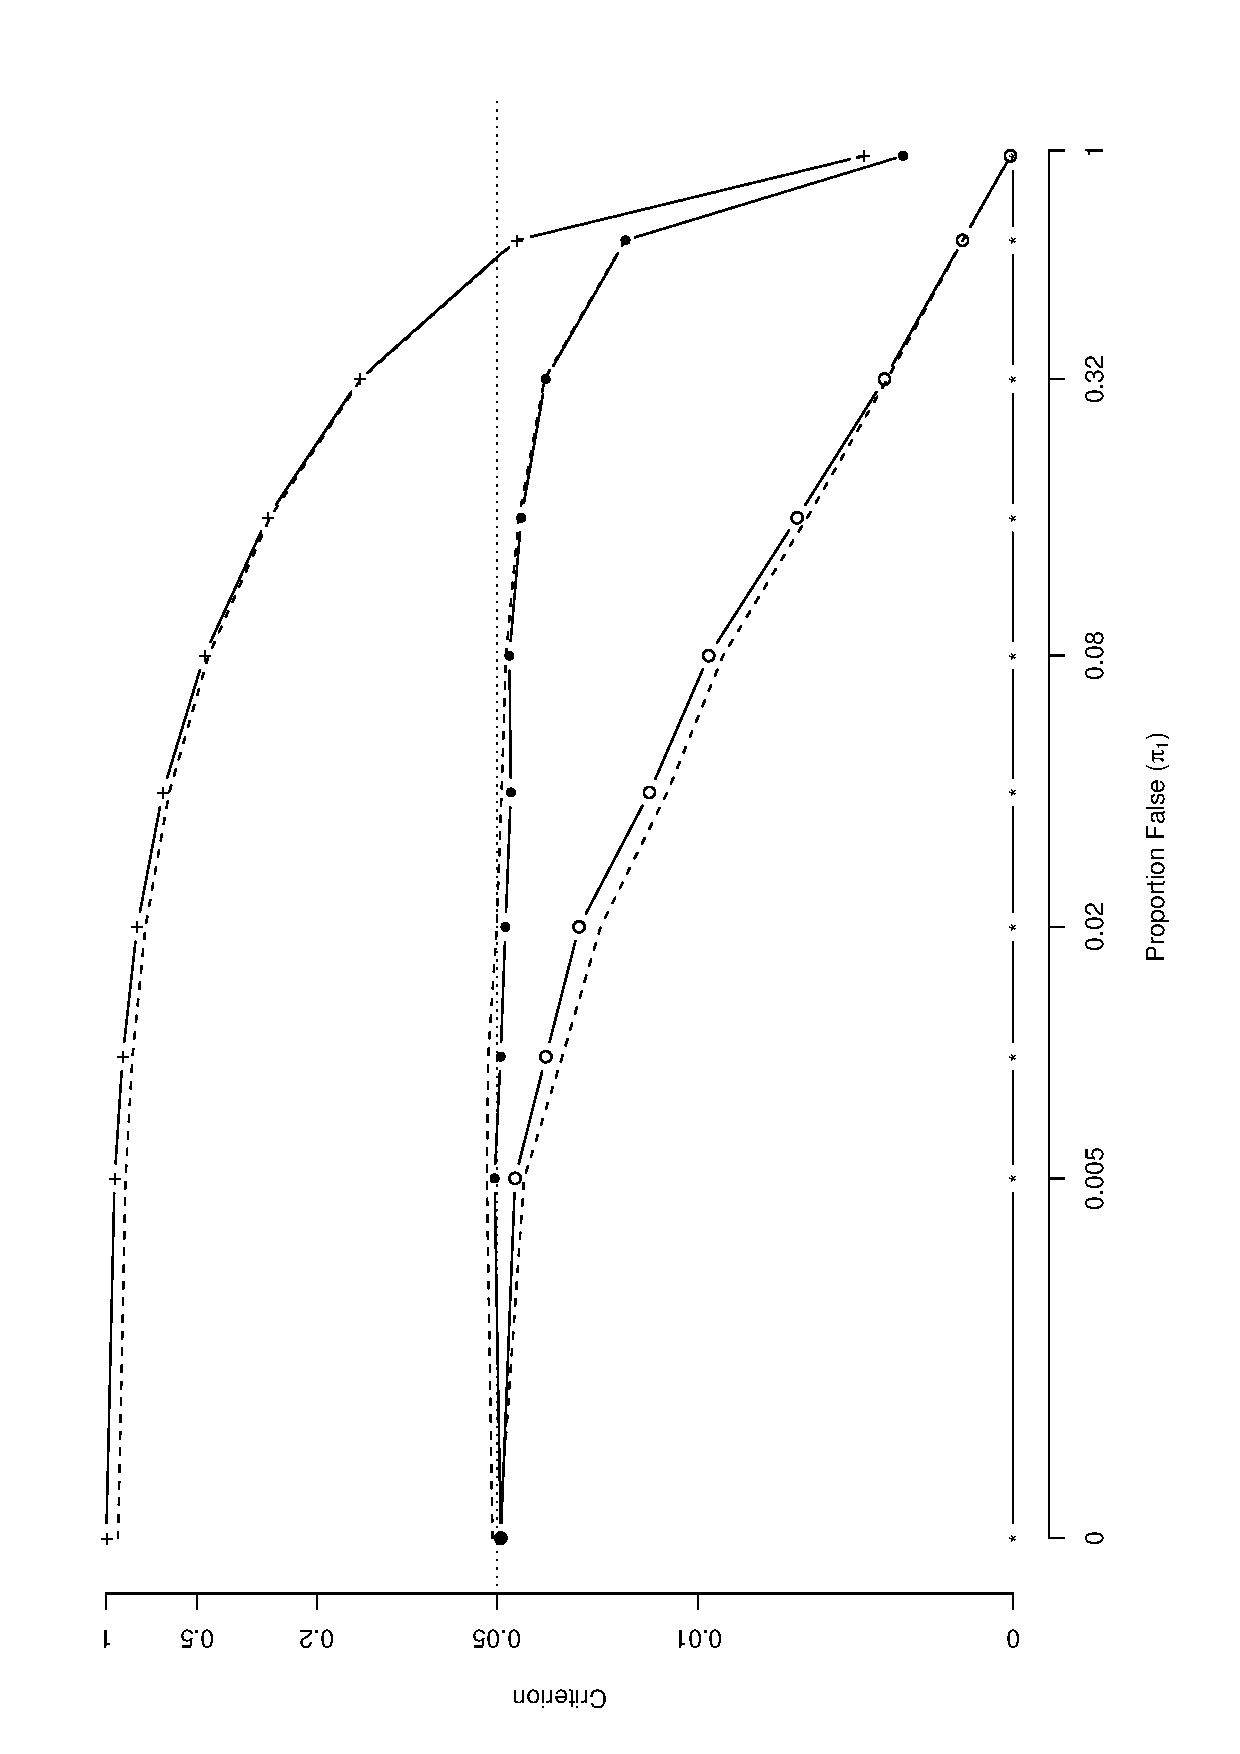
\includegraphics[width=4.5in]{figure1} }
        
\end{figure}


\clearpage


 \begin{figure}
\caption{\sl Alpha-investing design for testing two primary hypotheses $H_1$ and
 $H_2$ and two secondary hypotheses $H_3$ and $H_4$.  Shaded nodes indicate the
 path followed in the example; the data reject $H_1$ and $H_3$.}
\label{fi:example2}
\begin{center}
\ptbegtree
\ptnodefont{\normalsize\rm}{9pt}{1pt}
\ptleaffont{\normalsize\rm}{9pt}{1pt}

  \ptbeg
    \ptnode{\scriptsize $W(0) = 0.05$ }
    \ptbeg

      \ptnode{\hypy{1}{0.025}}
      \ptbeg
        \ptnode{\scriptsize $W(1) = 0.025$ }
        \ptbeg
          \ptnode{\hypn{2}{0.025}}
            \ptleaf{\scriptsize $W(2) = 0$}
          
            \ptbeg
              \ptnode{\scriptsize $W(2) = 0.05$}
              \ptbeg
                \ptnode{\hypn{3}{0.025}}
          
                  \ptbeg \ptnode{\scriptsize $W(3) = 0.025$} \ptnode{\hypn{4}{0.025}} \ptend
                  \ptbeg \ptnode{\scriptsize $W(3) = 0.075$} \ptnode{\hypn{4}{0.075}} \ptend
               
             \ptend
          \ptend
        \ptend
      \ptend
   

      \ptbeg
        \ptnode{\scriptsize $W(1) = 0.075$ }
        \ptbeg
          \ptnode{\hypy{2}{0.025}}

            \ptbeg
              \ptnode{\scriptsize $W(2) = 0.05$}
              \ptbeg
                \ptnode{\hypy{3}{0.025}}
          
                  \ptbeg \ptnode{\scriptsize $W(3) = 0.025$} \ptnode{\hypn{4}{0.025}} \ptend
                  \ptbeg \ptnode{\scriptsize $W(3) = 0.075$} \ptnode{\hypy{4}{0.075}} \ptend
               
              \ptend
            \ptend
          
            \ptbeg
              \ptnode{\scriptsize $W(2) = 0.10$}
              \ptbeg
                \ptnode{\hypn{3}{0.05}}
          
                  \ptbeg \ptnode{\scriptsize $W(3) = 0.05$} \ptnode{\hypn{4}{0.05}} \ptend
                  \ptbeg \ptnode{\scriptsize $W(3) = 0.10$} \ptnode{\hypn{4}{0.10}} \ptend
               
              \ptend
           \ptend
        \ptend
      \ptend

   \ptend
   \ptend
\ptendtree
\end{center}

\end{figure}


\end{document}
